\section{Sprachmodelle}

    \subsection{Überblick}
    	In diesem Abschnitt sollen die theoretischen Aspekte der Wortvorhersage erleutert werden. Es handelt sich hier um das Themengebiet des \emph{Natural Language Processing}. In diesem Abschnitt werden dazu ausschließlich Sprachmodelle behandelt. Um Annahmen darüber zu machen, welche Wörter nach einem anderen folgen können, benötigt man zunächst einmal ein Modell der verwendeten Sprache. Im optimalen Fall kann ein \emph{Sprachmodell} eine Sprache und die Beziehung zwischen Wörtern umfassend abbilden. In \autoref{sec:design-learnerPredictor} wird ein \emph{Sprachmodell} als Sammlung von Dateien mit Informationen über einen Text definiert. In diesem Abschnitt geht es um die Bedeutung dieser Informationen.
        
        Eine naheliegende Möglichkeit ein Modell einer Sprache zu generieren ist das Formulieren einer \emph{Grammatik}. Hierbei wird versucht die sytaktischen Regeln einer Sprache zu definieren. Im entworfenen Prototypen spielen solche \emph{Grammatiken} keine Rolle. Darum werden diese nur sehr kurz erklärt.
        
        Ein Beispiel einer einfachen Grammatik ist in \autoref{fig:grammer} zu sehen. \texttt{S -> NP VP} beschreibt, dass ein Satz \texttt{S} aus einem \emph{Noun Phrase} \texttt{NP} und einem \emph{Verb Phrase} \texttt{VP} bestehen kann. Alle weiteren Regeln funktionieren entsprechend. Mit Hilfe einer solchen Grammatik ist es möglich die Funktion eines Wortes innerhalb von einem Satz zu bestimmen. Dieser kann dann, wie in \autoref{fig:parsingTree} zu sehen,  als \emph{tree} dargestellt werden. Im Beispiel gilt es zu beachten, dass \autoref{fig:grammer} nicht alle in \autoref{fig:parsingTree} enthaltenden Worte enthält und somit erst einmal nicht funktionieren würde.
        
        Folgen wir also folgender vereinfachten Regel: Innerhalb eines \emph{Preposition Prase} \texttt{PP} nach einer Preposition \texttt{P} und einem Determinator \texttt{DET} muss immer ein Nomen \texttt{N} kommen. Dann können wir in dem Satzteil \texttt{in the …} aus \autoref{fig:parsingTree} nur noch Nomen als Folgewort vorschlagen.
        
        \begin{figure}[H]
			\centering
            \begin{subfigure}{0.49\textwidth}
				\begin{lstlisting}
S -> NP VP
VP -> V NP | V NP PP
PP -> P NP
V -> "saw" | "ate" | "walked"
NP -> "John" | "Mary" | "Bob" | Det N | Det N PP
Det -> "a" | "an" | "the" | "my"
N -> "man" | "dog" | "cat" | "telescope" | "park"
P -> "in" | "on" | "by" | "with"
    			\end{lstlisting}
                \caption{Einfache Grammatik}
                \label{fig:grammer}
			\end{subfigure}
            \begin{subfigure}{0.49\textwidth}
            	\centering
            	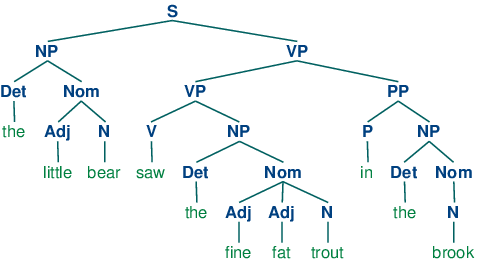
\includegraphics[width=.8\linewidth]{images/grammer.png}
            	\caption{\emph{parsing tree}}
            	\label{fig:parsingTree}
            \end{subfigure}
            \label{fig:grammerWithTree}
            \caption{Beispiel einer einfachen \emph{Grammatik} \parencite[Kapitel 8]{nltk:book}}
        \end{figure}
        \newpage
        
        Allerdings stößt man, wie von \cite[S. 544]{jamia:introduction} im Abschnitt \emph{The limitations of hand-written rules: the rise of statistical NLP} aufgefürht wird, mit solchen \emph{Grammatiken} an Grenzen. In dem Artikel werden zwei Probleme solcher \emph{Grammatiken} beschrieben.
    
    	Zum einen beschreiben diese in erster Linie Syntax und nicht die Semantik eines Satzes. Dies kann laut \cite{jamia:introduction} zwar durch Erweitern der Regeln gelöst werden. Sie Nutzen hier das Beispiel, dass das Verb \texttt{essen} nur für bestimmte \emph{essbare} Nomen gültig gemacht werden kann. Weißen aber darauf hin, dass so die Regeln viel zu komplex und unüberschaubar würden.
        
        Als zweites Problem führen sie an das solche \emph{Grammatiken} mit Sätzen, die zwar von Menschen verstanden werden aber nicht unbedingt grammatischen Regeln folgen, nicht umgehen können.
        
        \cite{jamia:introduction} beziehen sich bei Ihren Überlegungen, auch wenn sie Anwendungsbeispiele aus der Medizin nutzen, auf \emph{Natural Language Processing} im Allgemeinen. Hier soll versucht werden diese Formulierungen bezüglich der Wortvorhersage Teile zu verwenden.
        
        Aufgrund der genannten Probleme gab es, wie \cite{jamia:introduction} auf Seite 545 schließen, in den 1980ern eine Wende hin zu \emph{statistischem Natural Languge Processing}. Sie erklären \enquote{[\dots]fewer, broader rules replace numerous detailed rules, with statistical-frequency information looked up to disambiguate.} Übersetzt meinen sie also, dass weniger aber weiter gefasste Regeln in Kombination mit statistischen Frequenzen detaillierte Regeln ersetzen. Ein Beispiel für solche statistische Modelle sind die in \autoref{sec:n-gramms} erklärten \emph{N-gramms}.
        
        Ein statistisches Modell basiert immer auf Wahrscheinlichkeiten. Im gleichen Abschnitt beschreiben \cite{jamia:introduction} auch, dass diese Wahrscheinlichkeiten abhängig sind von dem Text aus welchem die Statistiken generiert werden. So liefert vereinfacht Formuliert eine auf Prosa Texten gelernte Statistik keine guten Ergebnisse auf Wissenschaftliche Texte.  
        
    \newpage
    \subsection{N-gramms}
    \label{sec:n-gramms}
    
    	Um Informationen über ein Wort in einem Text zu erhalten ist eine Möglichkeit sich die Umgebung dieses Wortes anzusehen. Ein \emph{N-gramm} besteht also aus einem Wort und den \emph{N-1} vorherigen Wörtern an einer Textstelle. Mit diesen Informationen können wir auch eine Sprache so beschreiben, dass wir Wortvrhersagen machen können. Brown u. a. machen dazu die in \autoref{eq:wordChain} \parencite[S. 468, Gleichung 1]{cumpatationalLinguistics:classBasedNGramms} gezeigte Annahme.
        
        \begin{equation}
        	Pr(w_1^k) = Pr(w_1) Pr(w_2|w_1) \cdots Pr(w_k|w_1^{k-1})
        	\label{eq:wordChain}
        \end{equation}
        
        Sie betrachten also die Wahrscheinlichkeit eines Wortes abhängig von seinen Vorgängern \(Pr(w_k|w_1^{k-1})\). Und definieren die Wahrscheinlichkeit einer Wortkette \(Pr(w_1^k)\) als Summe dieser Wahrscheinlichkeiten. In dem online Buch \parencite{nlwp:book} wird dazu unter Abschnitt 3.8 eine gute Erklärung geliefert. Zunächst formulieren de Kok und Brouwer die Formel neu mit einem Beispielsatz. Hier wird dazu in \autoref{eq:wordChainWithWords} der Satz \texttt{the cat chased the mouse} verwendet werden.
        
        \begin{equation}
        	\begin{split}
        		Pr(\text{the cat chased the mouse}) \\
                = Pr(\text{the}) Pr(\text{cat}|\text{the}) Pr(\text{chased}|\text{the cat}) \\
                Pr(\text{the}|\text{the cat chased}) Pr(\text{mouse}|\text{the cat chased the}) 
            \end{split}
            \label{eq:wordChainWithWords}
        \end{equation}
        
        Im gleichen Abschnitt erklären sie, dass ein \emph{korrekter} Satz eine höhere Wahrscheinlichkeit haben wird als ein fehlerhafter. Interessant ist hier was als \emph{korrekt} verstanden wird. Da sich diese Wahrscheinlichkeiten auf aus Trainingstexten gelernten Statistiken beziehen. So kann ein viel verwendeter grammatisch unkorrekter Satz auch eine hohe Wahrscheinlichkeit haben. Das ist eine durchaus erwünschte Eigenschaft solcher Modelle.
        
        In \parencite{nltk:book} unter Abschnitt 1.1 von Kapitel 8 wird sehr schön gezeigt, dass es theoretisch unendlich solcher \emph{korrekter} Sätze gibt. Es ist also unmöglich, selbst mit sehr großen Trainingstexten eine Sprache komplett abzubilden und mit \autoref{eq:wordChain} für jeden denkbaren Satz Wahrscheinlichkeiten zu berechnen. 
        
        De Kok und Brouwer erwähnen auch, dass es sich bei \autoref{eq:wordChain} um eine Markow-Kette handelt. Sie fahren fort, dass wir auf die Kette nun auch die Markow-Annahme anwenden können. Diese formulieren sie übersetzt als: \enquote{Die Vorhersage des nächsten Zustands ist nur Abhängig von dem aktuellen Zustand.}\parencite[Abs.  3.8]{nlwp:book}
        
        \autoref{eq:markov-assumtion} zeigt \parencite[Abs.  3.8, Gleichung 3.8]{nlwp:book} in leicht veränderter Schreibweise um innerhalb dieser Arbeit konsitente Bezeichnungen zu verwenden.  
        
        \begin{equation}
        	Pr(w_k|w_1^{k-1}) \approx Pr(w_k|w_{k-1})
        	\label{eq:markov-assumtion}
        \end{equation}
        
        Dieses vereinfachte Modell nennt sich \emph{bigramm} Modell. Die übergangswahrscheinlickeit von \(w_{k-1}\) nach \(w_k\) lässt sich einfach mit \autoref{eq:bigramm-prob} berechnen. Dabei handelt es sich um \parencite[Abs.  3.8, Gleichung 3.9]{nlwp:book} wieder mit angepasster schreibweise. Damit ist es auch möglich Wortvorhersagen zu treffen.
        
        \begin{equation}
        	Pr(w_k|w_{k-1}) = \frac{C(w_{k-1};w_k)}{C(w_{k-1})}
        	\label{eq:bigramm-prob}
        \end{equation}
    	
    	\(C(w_{k-1};w_k)\) gibt an wie oft im Trainingstext das Wort \(w_{k-1}\) direkt vor \(w_k\) steht. \(C(w_{k-1})\) ist die Häufigkeit des Wortes \(w_{k-1}\) im Trainingstext.
        
        
        Es ist möglich die Qualität der Vorhersage zu verbessern, wenn man nun nicht nur das vorherige Wort sondern die zwei vorherigen Worte betrachtet. Oder auch, sich \autoref{eq:wordChain} wieder annähernd, die \(N - 1\) vorherigen Worte. Umso größer \emph{N} jedoch wird desto unwahrscheinlicher wird es, dass ein \emph{N-gramm} auch im Trainingstext vorkommt. So werden die Kombinationen \texttt{ich bin} und \texttt{ich war} in einem ausreichend großem Text oft genug vorkommen um gute Aussagen über ihre Wahrscheinlichkeit machen zu können. Bei einer Kombination \texttt{ich war gestern abend} ist schon ein einmaliges Vorkommen nicht unbedingt gegeben.
        
        Da diese Wahrscheinlichkeiten mit Hilfe eines Trainingstextes angelernt werden, besteht die Gefahr, dass das Modell zu stark auf die Trainingsdaten abbildet.
        
        -> smoothing (small frequencis are oberrepresnted)
        -> overfitting -> predict excatly learned text but not real languge
        -> espacially bad of prediction is the only input method because you can't predict words that were not learned see evaluation
        
    \newpage
	\subsection{Klassenbasierte n-gramm Sprachmodelle}
    \label{sec:brownClustering}
    
    	-> exmple from brown: next Monday != next Thuesday
        -> is some kind of smoothing
        -> rertive cluster by assumtion:
    
    	\begin{equation}
   			P(w_i|w_{i-1}) = P(w_i|c_i) P(c_i|c_{i-1})
        	\label{eq:wordPropability}
		\end{equation}
        
        -> explain buttom up algorythm
        
    \newpage    
    \subsection{Corpora}
    	statistischre basieren auf -> corpora is text
        modell abhängig von corpora
    	Finanztext anders als Liebesbrief
        Nicht nur andere Haäfigkeiten sondern auch andere Vokabeln 
        
        -> kleine Corpora führen zu overfitting und beschränktem Wortschatz
        -> bedeutung für protytypen
    \newpage
    
